%\documentclass[10pt]{beamer}
%\usetheme{amcg}

%\begin{document}

\section{Flow past a sphere}

\frame{
  \frametitle{Flow past a sphere}
  \begin{itemize}
    \item Fluidity is used compute the drag force on an isolated sphere, see Chapter 10.7.2 and Equation (10.2) in the manual for more details.\newline
    %\begin{equation}
    %  \label{eq:drag_coefficient}
    %  C_D = \frac{F_x}{\frac{1}{2} \rho u_0^2 A}, \;\;\; \text{with} \;\;\; F_x = \int_S (n_x p - n_i\tau_{ix})dS
    %\end{equation}
    \item The results are compared against a curve optimised to fit a large amount of experimental data (Brown and Lawler, 2003), see Chapter 10.7.3 and Equation (10.3) in the manual for more details.\\
    %\begin{equation}
    %  \label{eq:drag_coefficient_brown2003}
    %  C_D = \frac{24}{Re}(1+0.15Re^{0.681}) + \frac{0.407}{1+\frac{8710}{Re}}
    %\end{equation}
  \end{itemize}
  
}

\frame{
  \frametitle{Flow past a sphere - Setup}
  \begin{itemize}
    \item The sphere is modelled as a void space in the mesh.\newline
    \item The flow is assumed to be incompressible\newline
    \item Free-slip boundary conditions are applied to the top, bottom and side walls, and a no-slip condition to the surface of the sphere.
  \end{itemize}
}

\frame{
  \frametitle{Flow past a sphere - Computational domain}
  \begin{figure}[h]
    \centering
    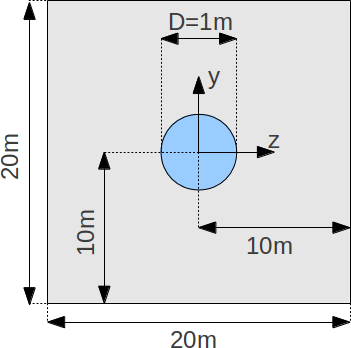
\includegraphics[scale=0.22]{flow_past_sphere/images/domain_yz.png}\quad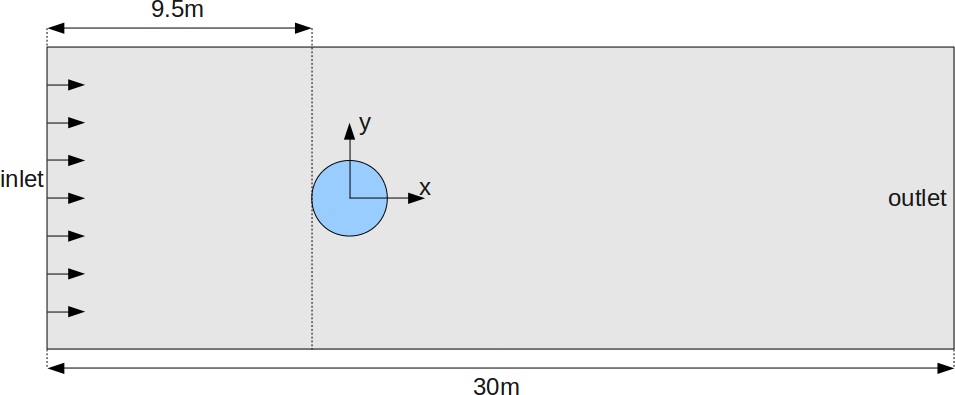
\includegraphics[scale=0.22]{flow_past_sphere/images/domain_xy.png}
  \end{figure}
}

\frame{
  \frametitle{Flow past a sphere - Results}
  \begin{figure}
  \centering
    \subfigure{
    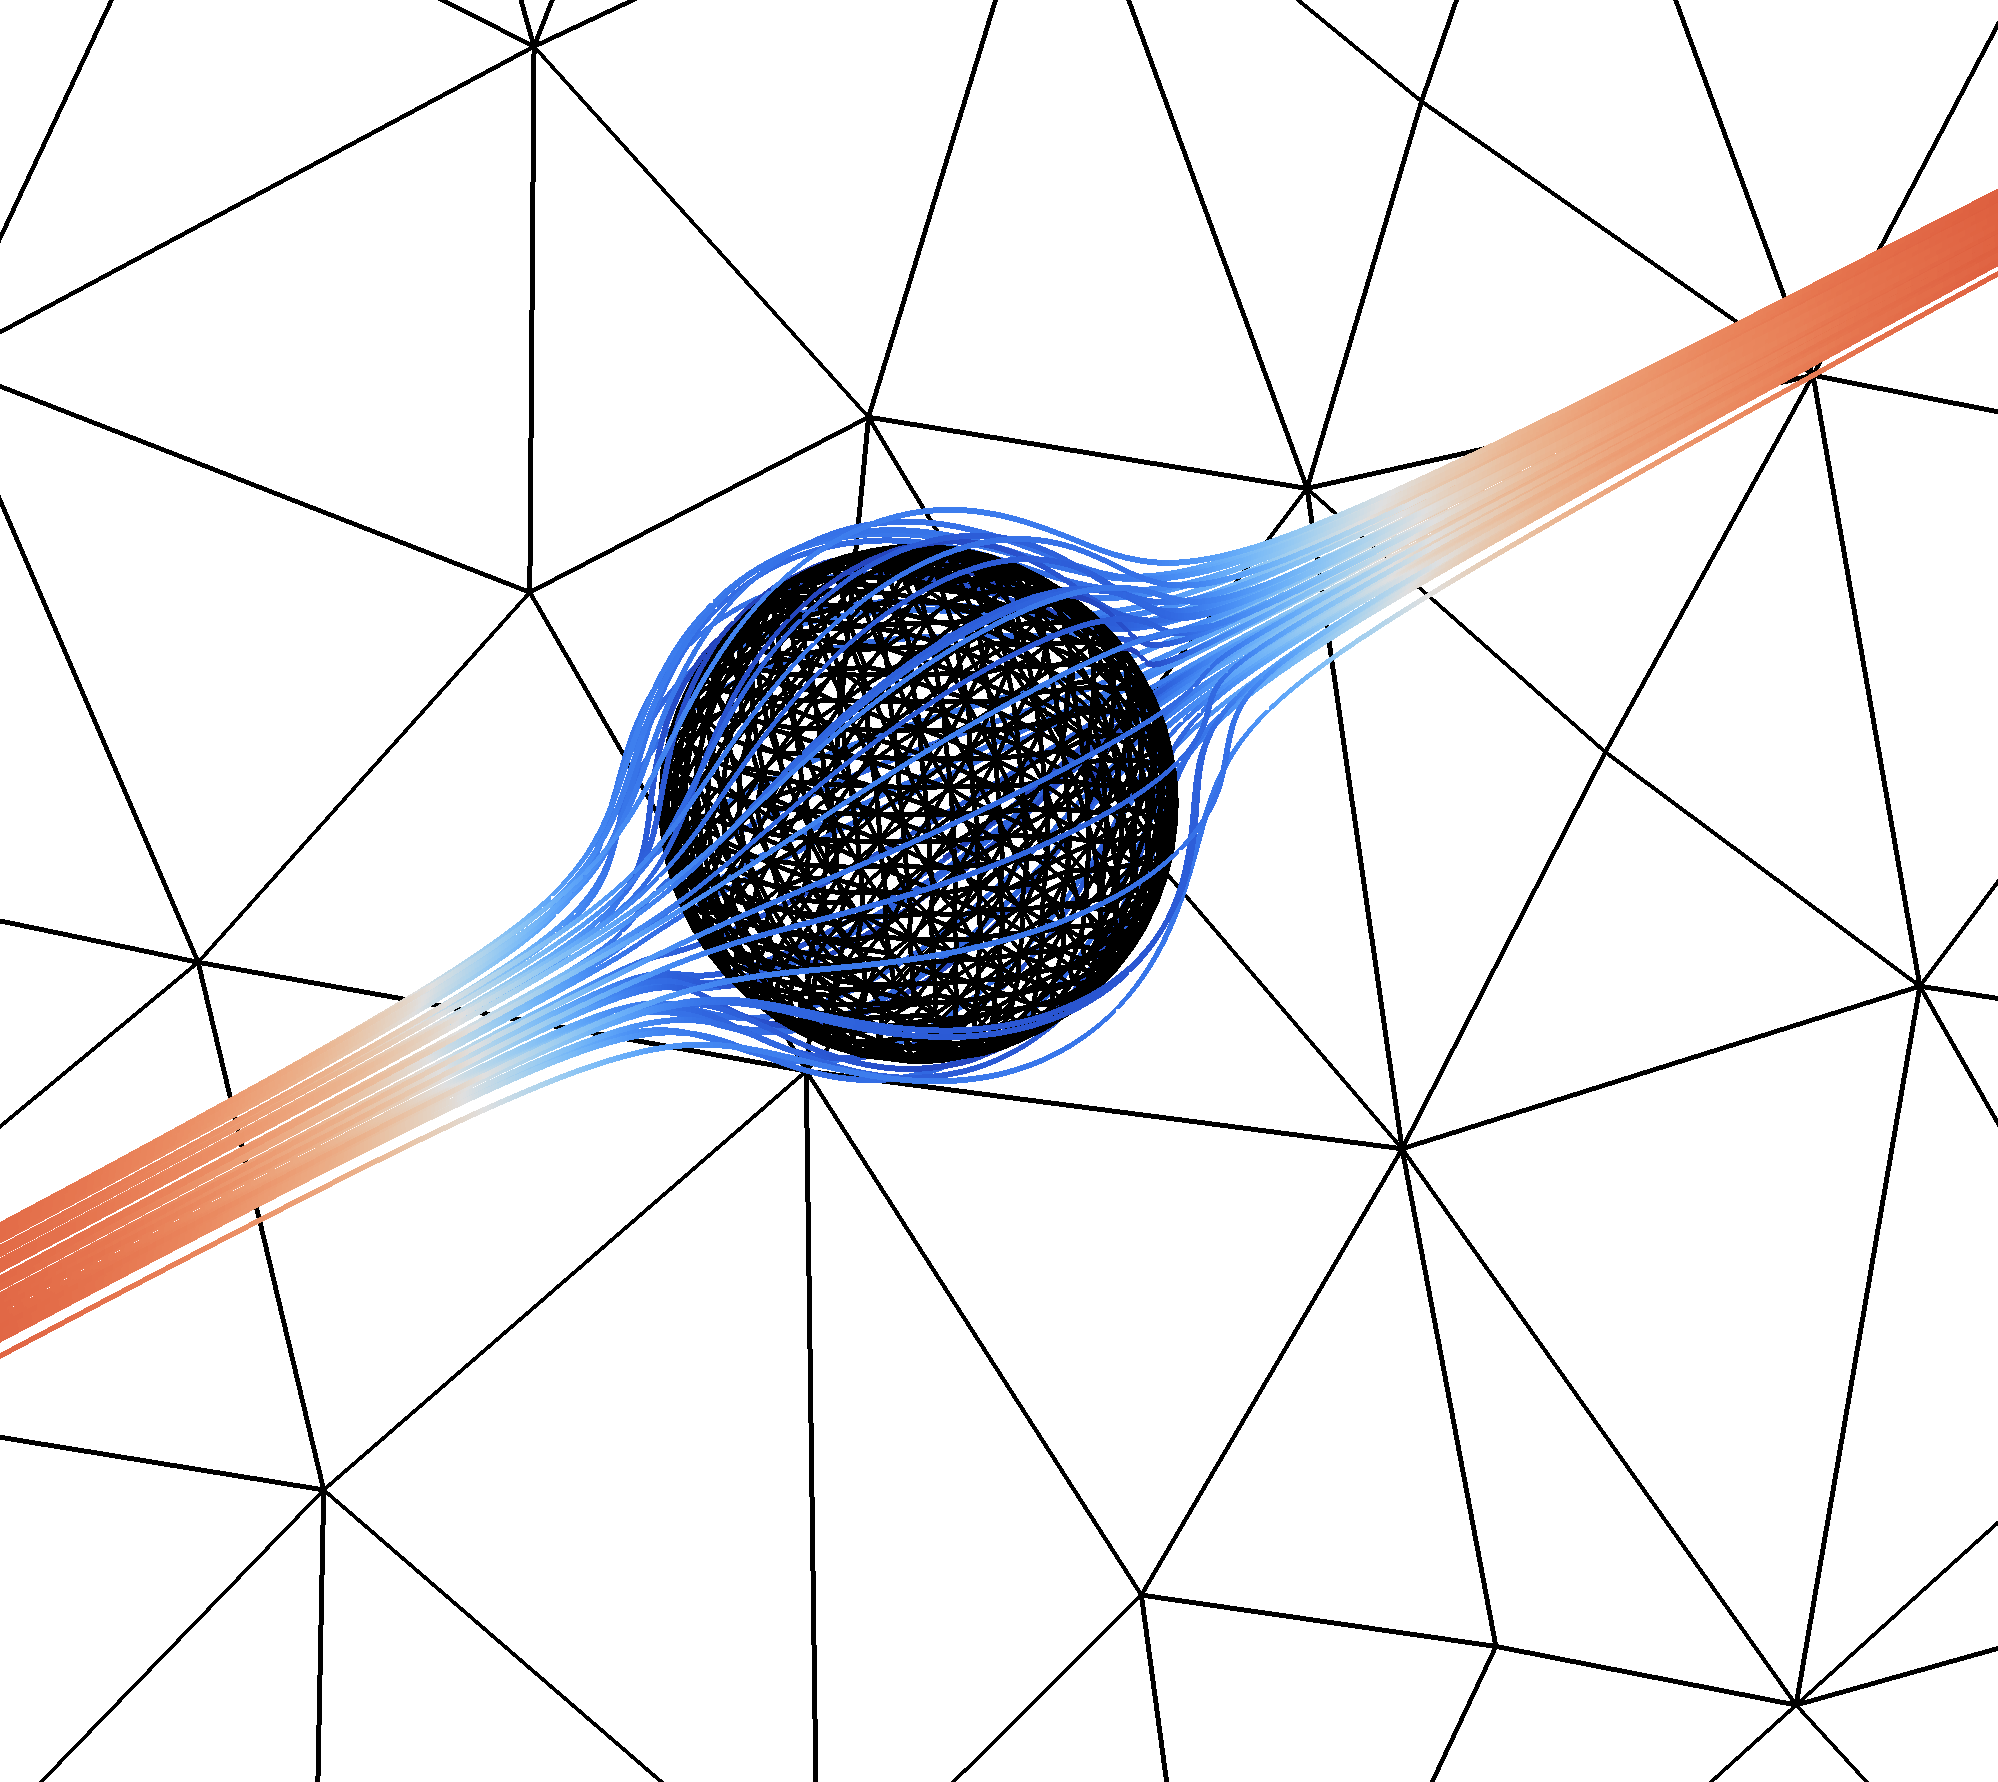
\includegraphics[scale=0.0425,clip]{flow_past_sphere/images/sphere-Re1-streamlines.png}}
    \subfigure{
    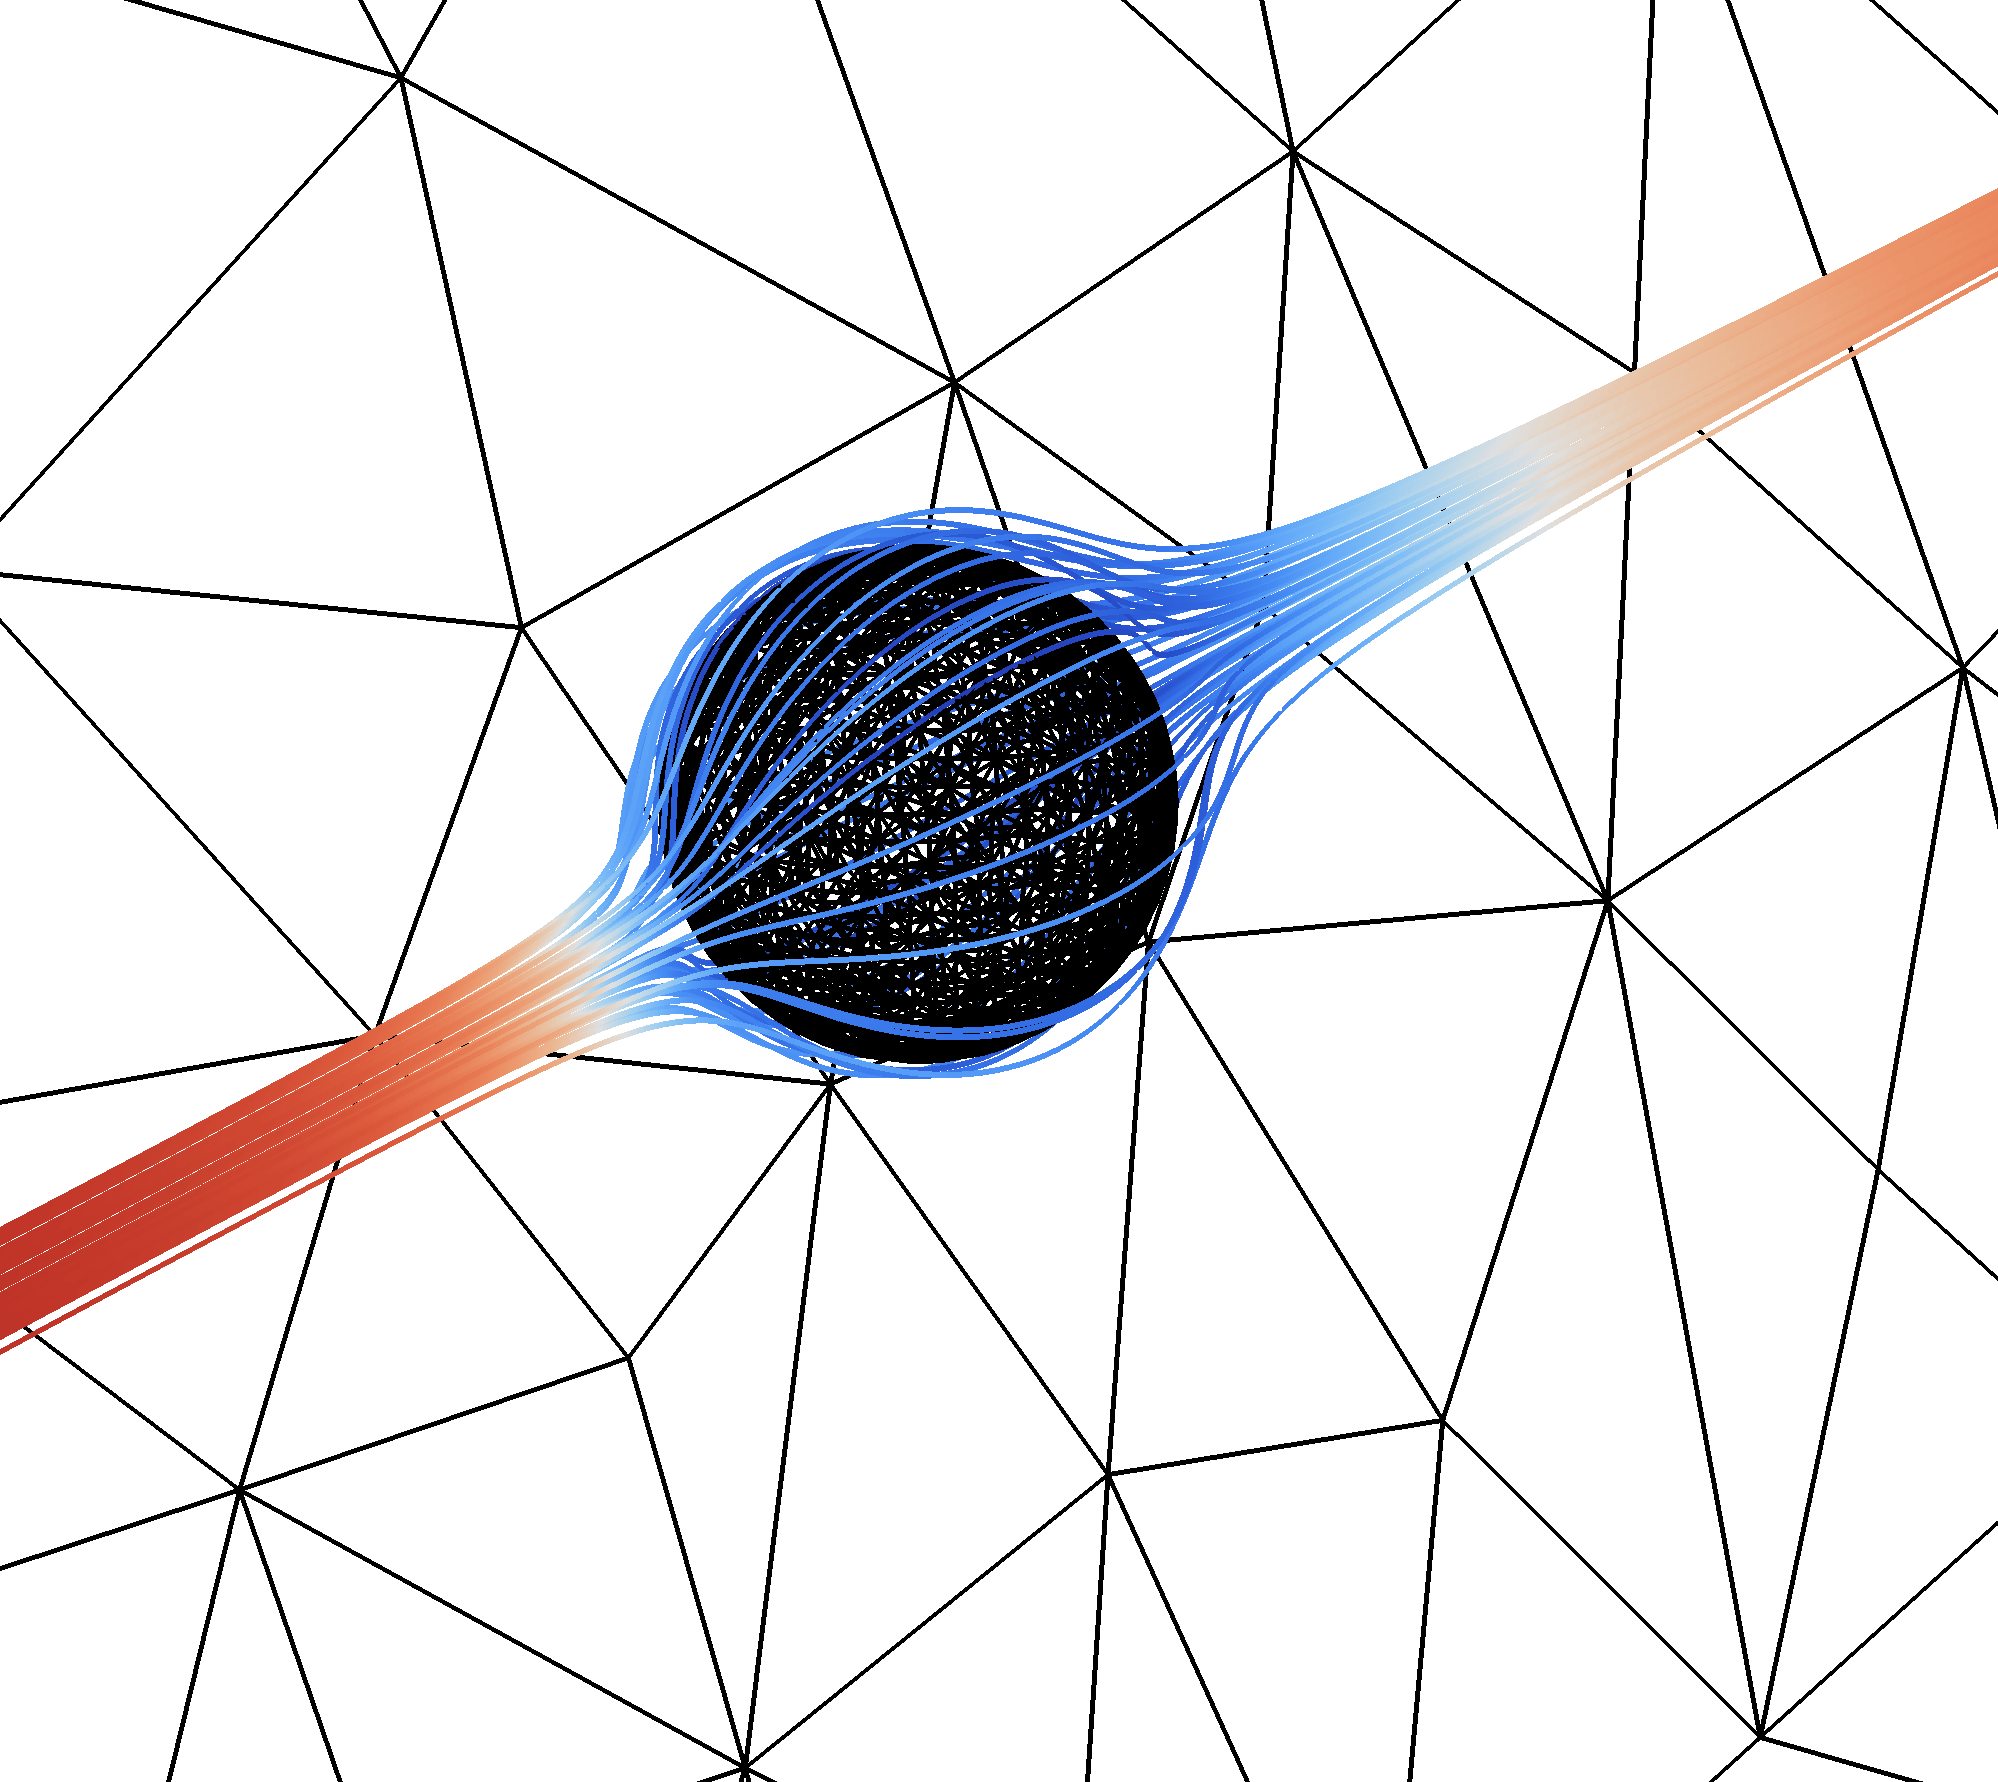
\includegraphics[scale=0.0425,clip]{flow_past_sphere/images/sphere-Re10-streamlines.png}}
    \\
    \subfigure{
    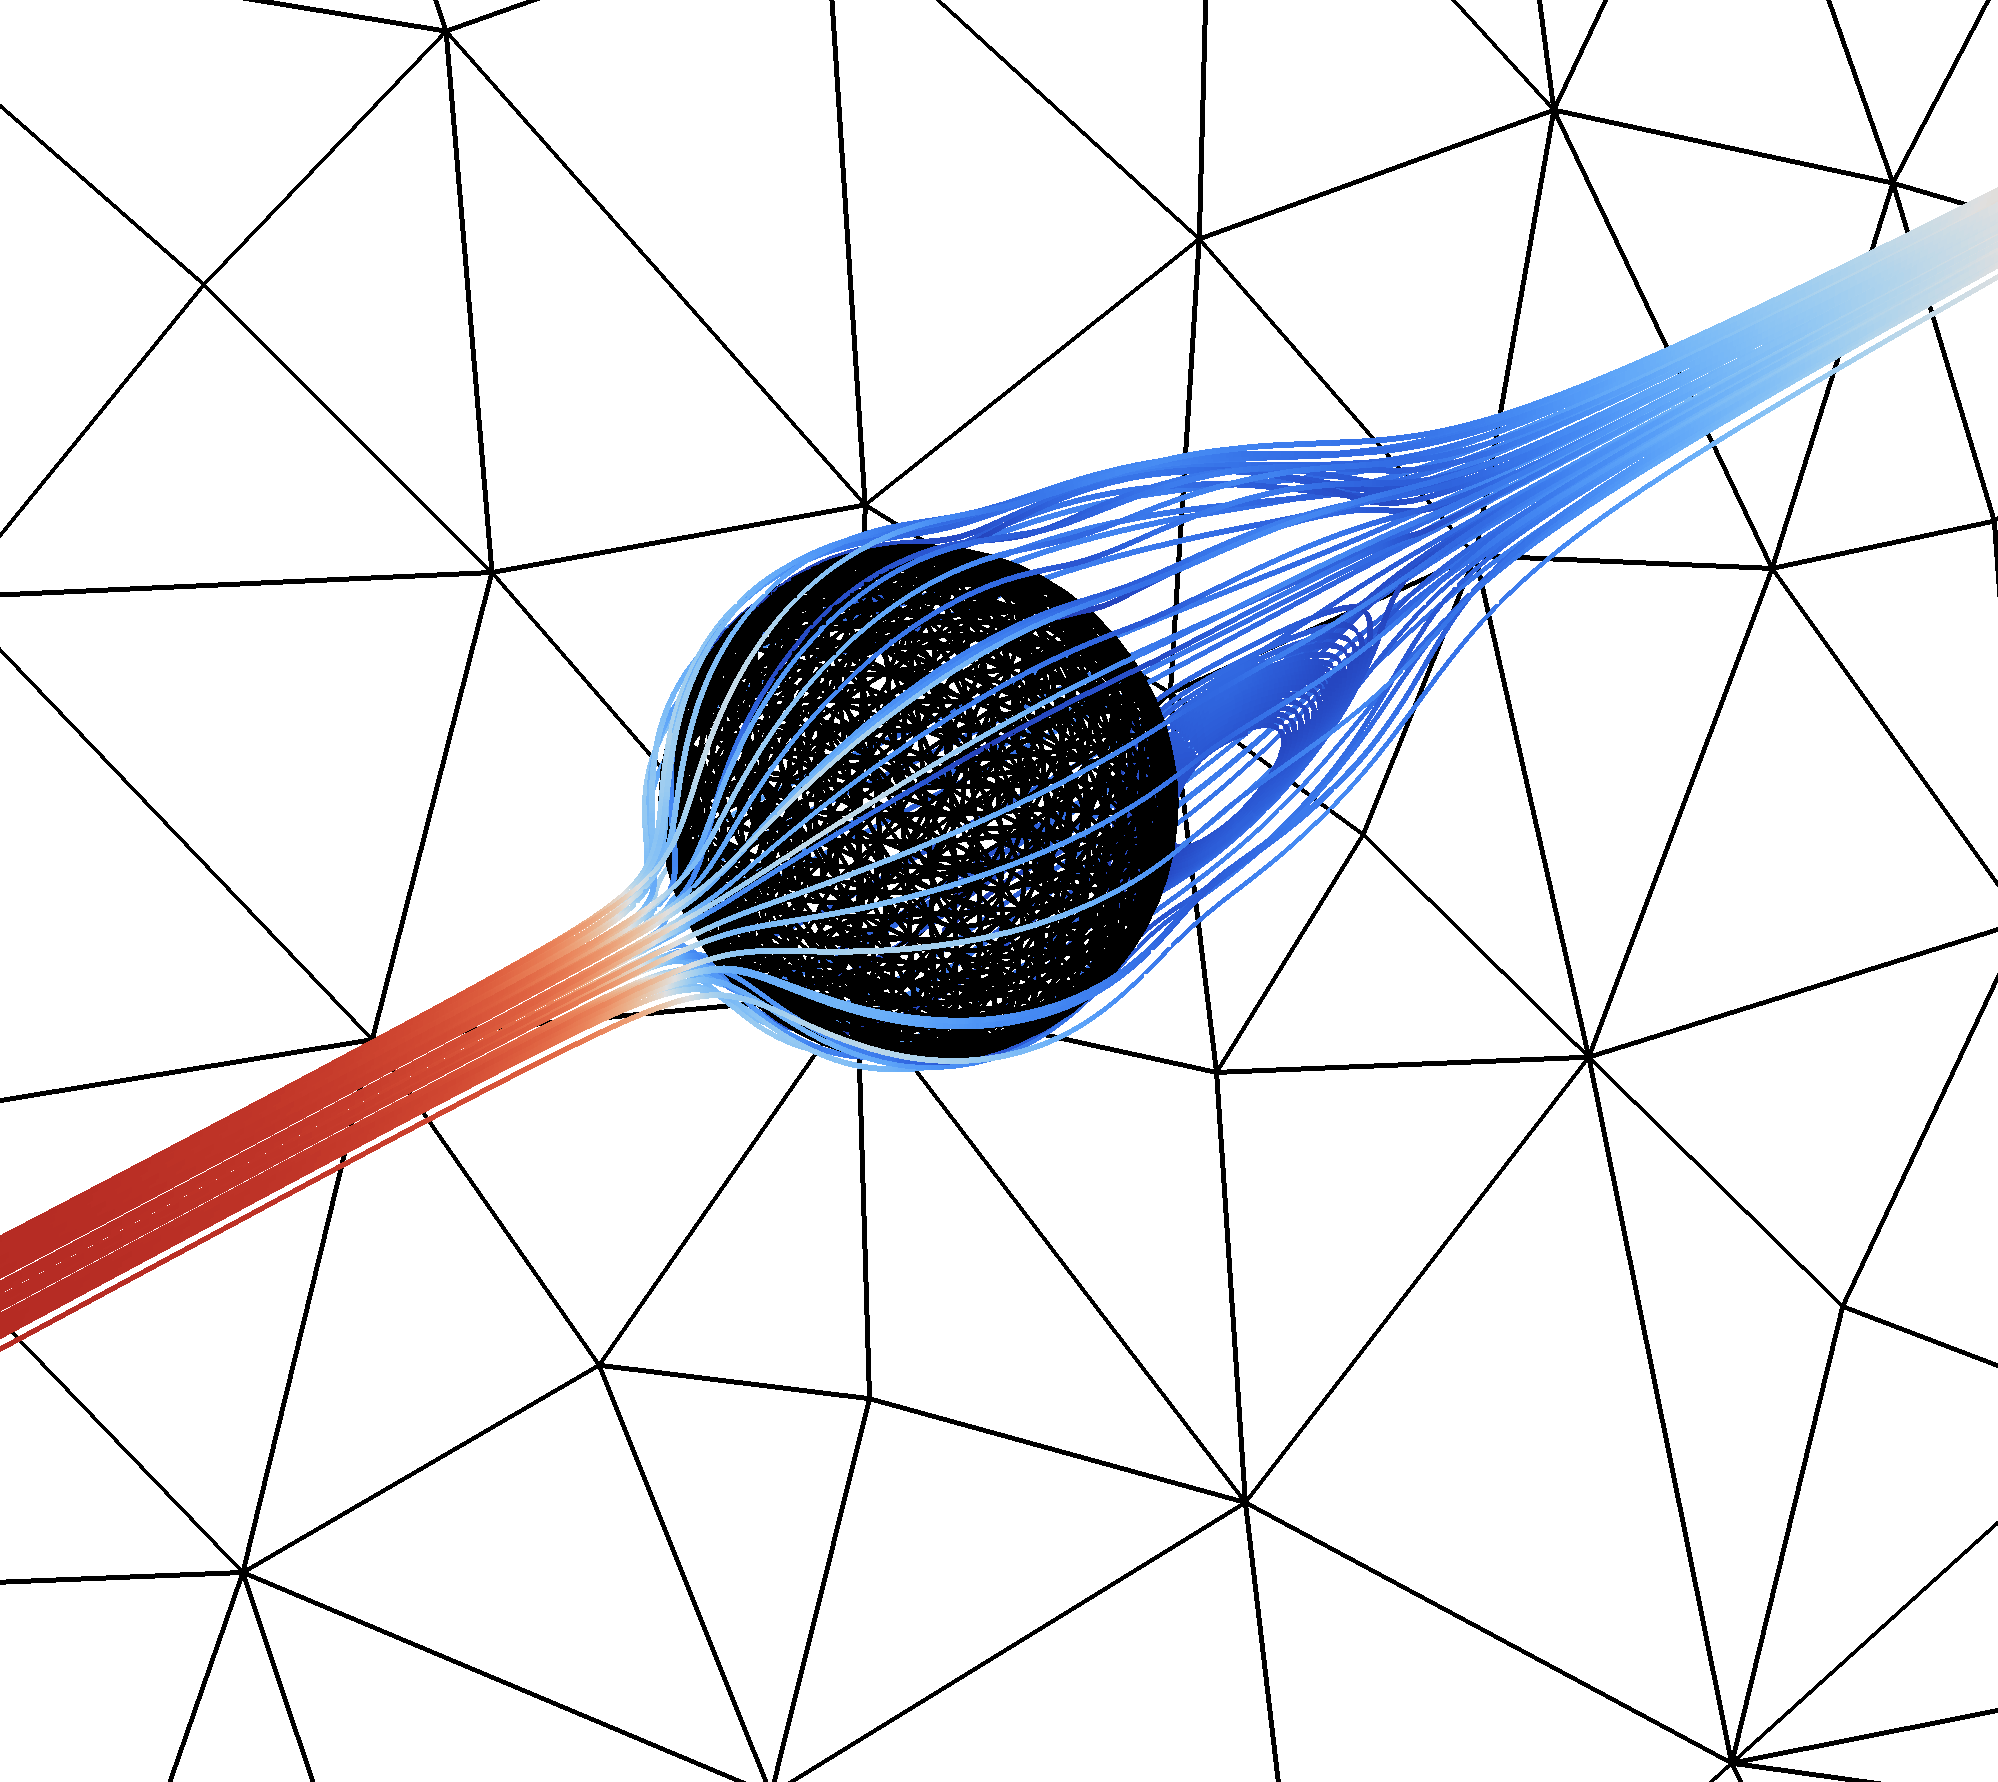
\includegraphics[scale=0.0425,clip]{flow_past_sphere/images/sphere-Re100-streamlines.png}}
    \subfigure{
    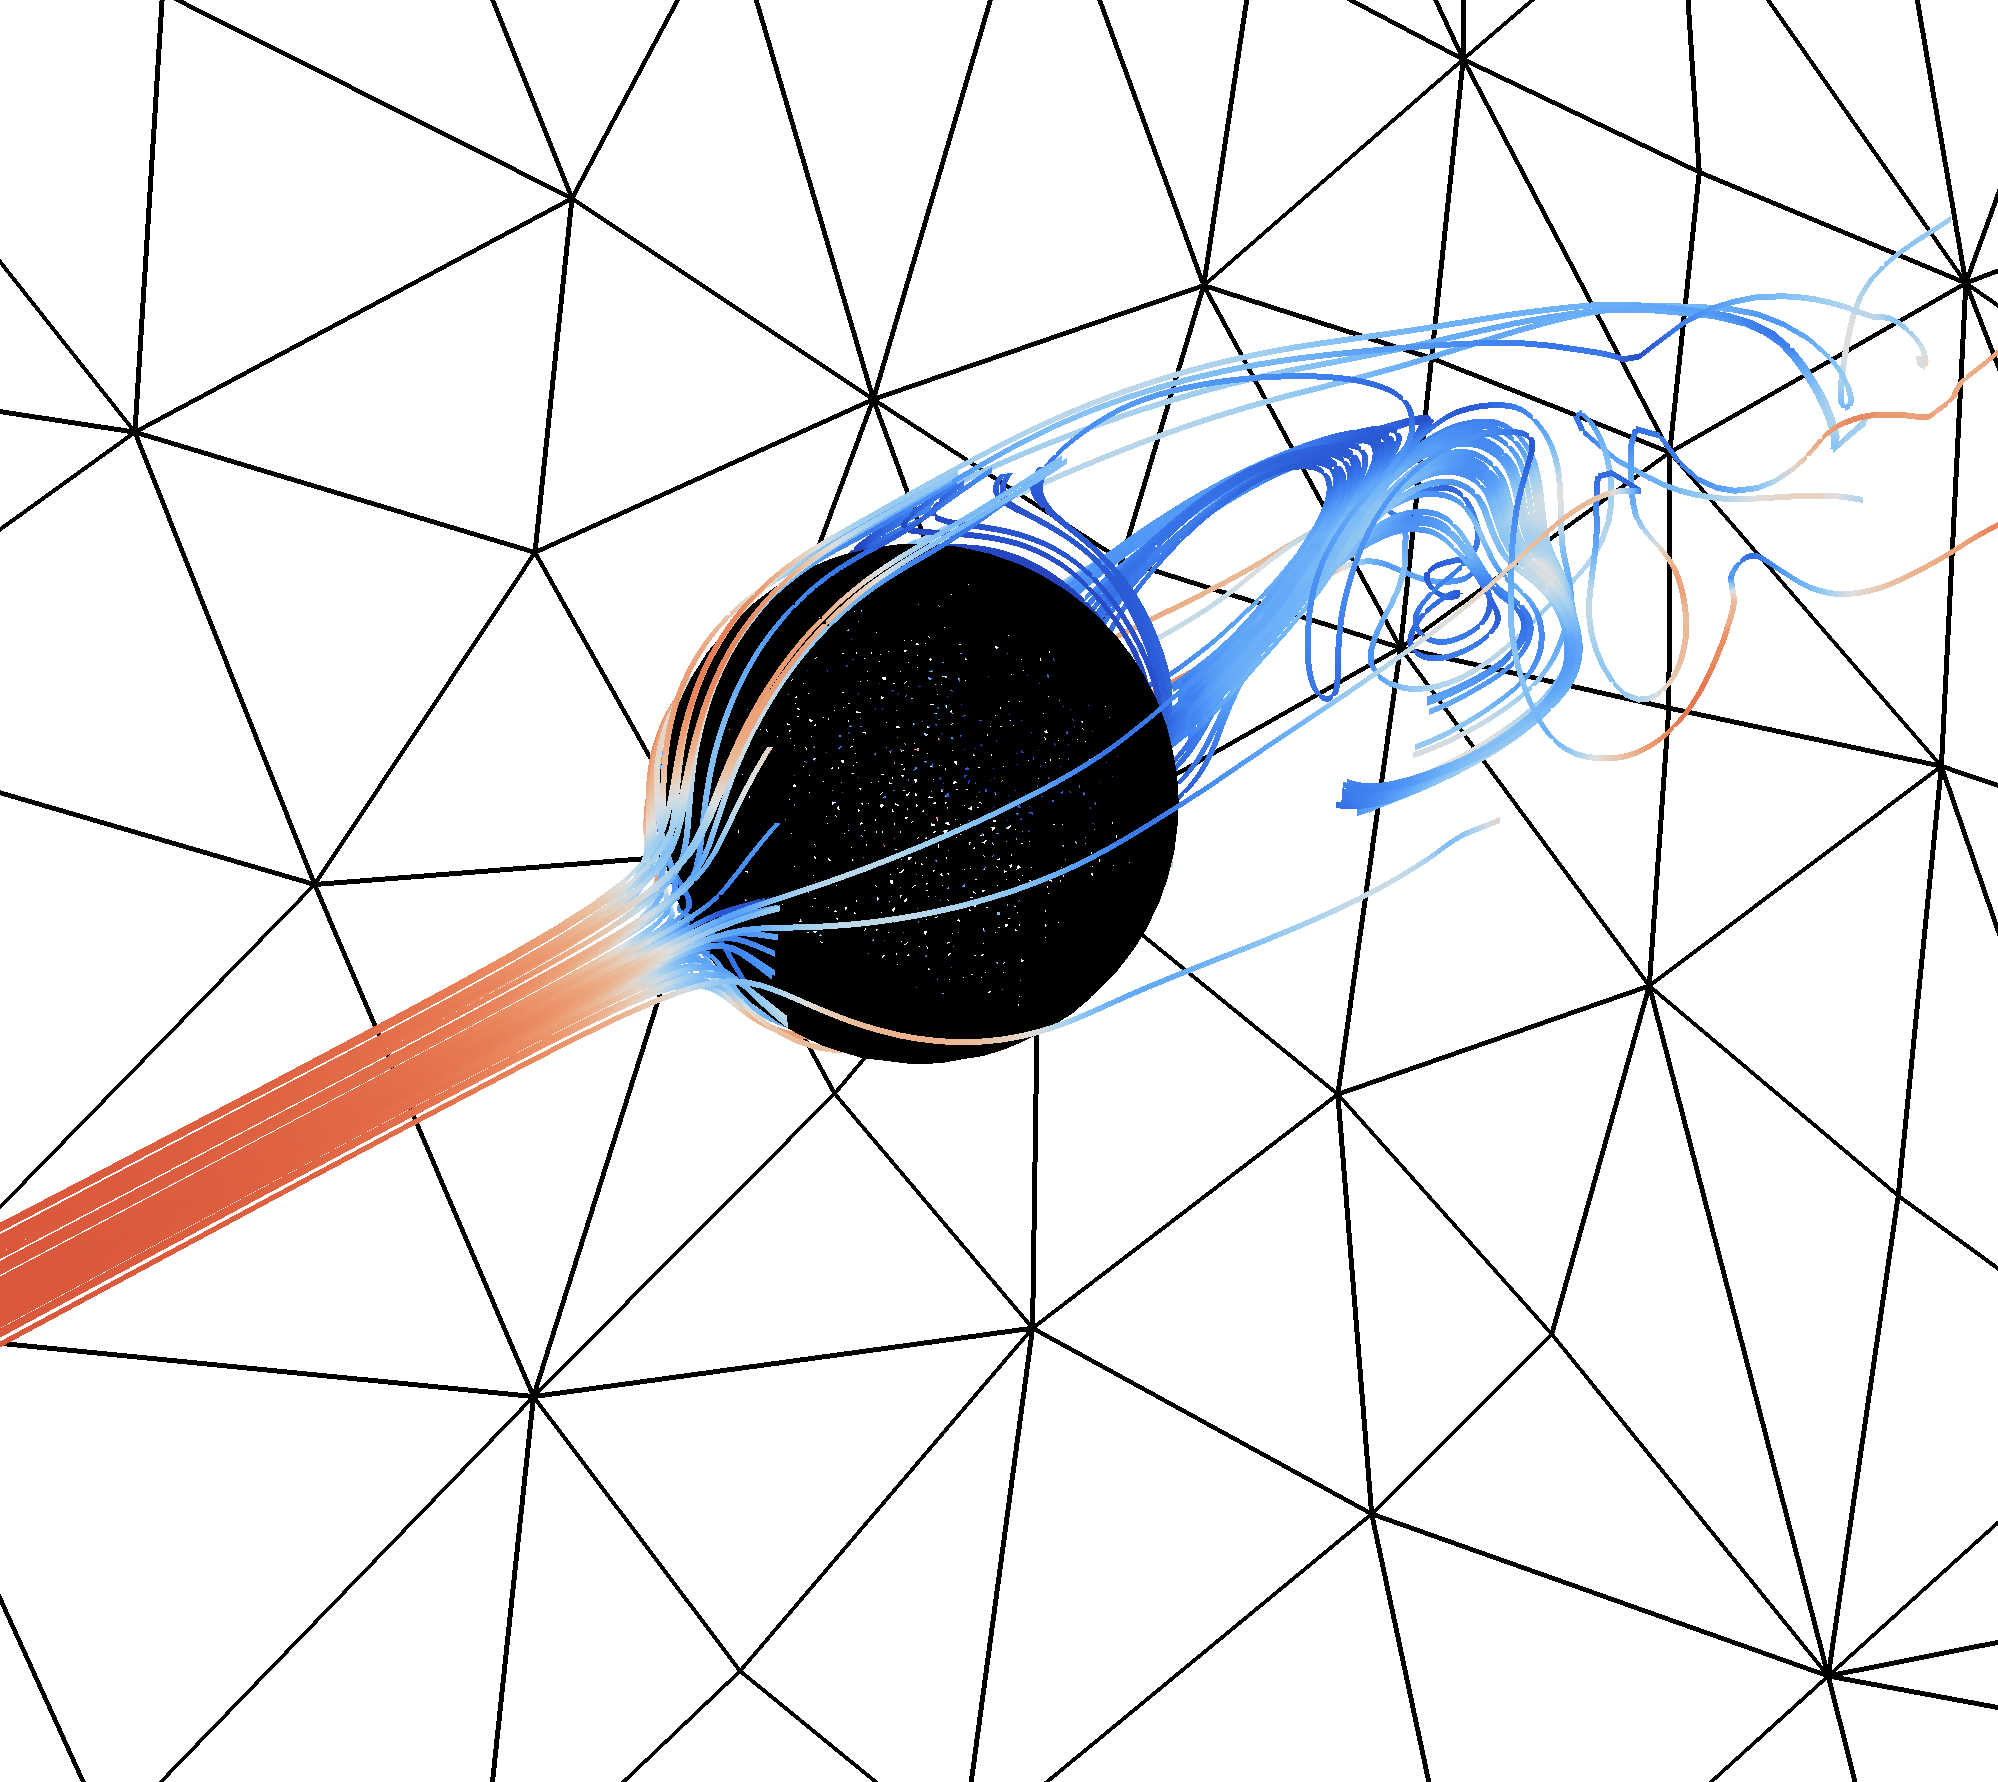
\includegraphics[scale=0.0425,clip]{flow_past_sphere/images/sphere-Re1000-streamlines.png}}
    \caption{Streamlines and surface mesh in the flow past the sphere example. Top-left to bottom-right
    show results from Reynolds numbers $Re=1,10,100,1000$.}
  \end{figure}
}

\frame{
  \frametitle{Flow past a sphere - Results}
  \begin{figure}
  \centering
  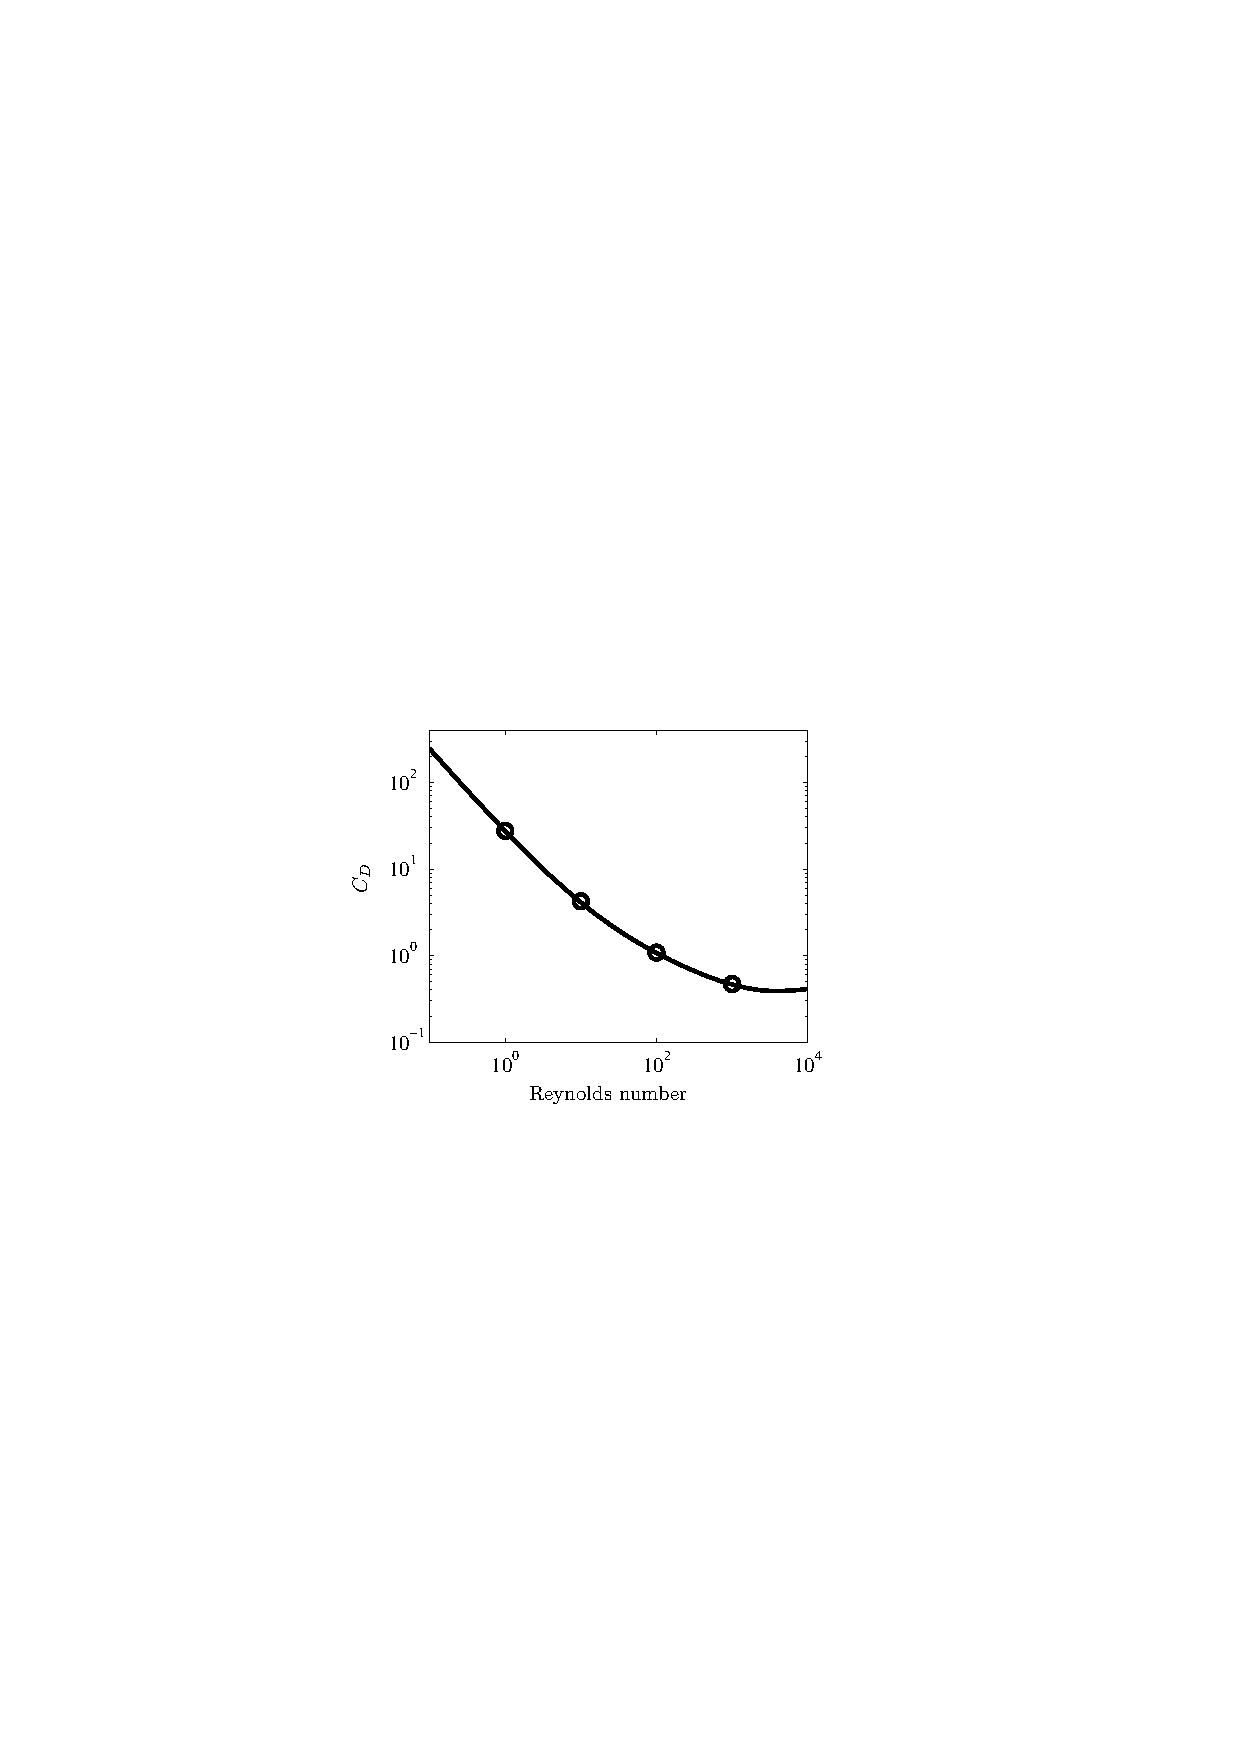
\includegraphics[scale=1]{flow_past_sphere/images/Sphere_Drag}
  \end{figure}
}

\frame{
  \frametitle{Flow past a sphere - Exercises}
  \begin{itemize}
    \item We actually compute the (vector) force on the sphere and output this to the stat file. This can then be converted to the drag coefficient via (10.2). Write a Python function to do this conversion and the error from the correlation (10.3).\newline
    \item Try varying some of the discretisation and adaptivity parameters to see what the impact on the accuracy of the calculated drag is.\newline
    \item Try changing the shape of the object, e.g.~benchmark data is also available for flow past a cylinder [Sch\"{a}fer et al., 1996].
  \end{itemize}
}

%\end{document}
